\documentclass[a4paper,12pt]{book}
\usepackage[utf8]{inputenc}
\usepackage[T1]{fontenc}
\usepackage{graphicx}
\usepackage[italian]{babel}
\usepackage{microtype}
\usepackage{lmodern}
%\usepackage{frontespizio}
%\pagestyle{headings}
\usepackage{fancyhdr}
\pagestyle{fancy}
\fancyhf{}
\fancyhead[CE,CO]{\leftmark}
\fancyfoot[CE,CO]{\thepage}
\usepackage[italian]{varioref}
\usepackage{float}
\usepackage{booktabs}
\usepackage{caption}
\captionsetup{tableposition=top,figureposition=bottom,font=small,format=hang,labelfont={sf,bf}}
\usepackage{graphicx}
\usepackage{rotating}
\usepackage{amsmath}
\usepackage{url}
\usepackage{hyperref}
\hypersetup{hidelinks}
\usepackage{version}
\usepackage{pdfpages}
\usepackage{listings}
\lstset{language=C}

\begin{document}
	\begin{titlepage}
		\centering
		{\scshape\huge Università degli Studi di Napoli Federico II \par}
		\vspace{1cm}
		{\scshape\large Dipartimento di Ingegneria Elettrica e delle Tecnologie dell'Informazione\par}
		\vspace{0.5cm}
		
		\vspace{1.5cm}
		{\bfseries\huge Impianti di Elaborazione\par}
		\vspace{0.5cm}
		{\ttfamily\Large Elaborato\par}
		%{\huge\bfseries Elaborato\par}
		\vspace{2cm}
		{\Large\itshape Michele Pommella\par}
		{\Large\itshape Davide Trimaldi\par}
		\vspace{1.5cm}
		{\large Prof.~Domenico Cotroneo\par}
		
		\vfill
		
		% Bottom of the page
		{\large Anno 2018-2019\par}
	\end{titlepage}

\tableofcontents
\listoffigures

\mainmatter
\chapter{Benchmark}
Il primo elaborato consta di un \emph{Linux I/O benchmark} per le operazioni di lettura e scrittura su di un file binario. Le dimensioni di file valutate sono:
\begin{itemize}
	\item $10MB$
	\item $100MB$
	\item $1GB$
\end{itemize}
Le operazioni di I/O avvengono a blocchi di dimensione:
\begin{itemize}
	\item $1KB$
	\item $10KB$
	\item $100KB$
	\item $1MB$
\end{itemize}
Il sistema utilizzato è composto da:
\begin{itemize}
	\item processore \texttt{Intel Celeron N3050} $1.60GHz$
	\item memoria RAM DDR3 $4GB$
	\item disco \texttt{HGST HTS545050A7} $500GB$
\end{itemize}
Sono stati effettuati $30$ esperimenti per ogni configurazione attraverso uno script \emph{bash}. Prima di ogni esperimento sono stati utilizzati i comandi \emph{sync} ed $echo\ 1 > /proc/sys/vm/drop\_caches$ per ottenere l'indipendenza tra essi (purge della cache).\par 
Si è sfruttata la direttiva \texttt{O\_DIRECT} all'apertura dei file, per minimizzare l'effetto della cache nelle operazioni di I/O da e verso il file. Ciò ha richiesto l'utilizzo di blocchi allineati, multipli di 512 byte, la cui creazione è stata demandata alla funzione \emph{posix\_memalign}. Il calcolo del tempo è effettuato con \emph{gettimeofday}, ed è attuato in microsecondi.

	\section{Lettura}
		Per effettuare le operazioni di lettura, si è sfruttato un unico file \emph{prova.bin} di $1GB$, creato in precedenza. Si sfruttano le direttive della primitiva \emph{open} che consentono la lettura del file e la lettura diretta dallo storage.
		\lstinputlisting[]{./codice/benchmarkI.c}
	
	\section{Scrittura}
		Le operazioni di scrittura sono effettuate sul file \emph{test.bin}, che viene creato, se già esistente, o altrimenti sovrascritto. Ciò è definito dalle direttive della primitiva \emph{open}, che inoltre indicano l'apertura in scrittura del file, da attuare direttamente verso lo storage. Nel caso di creazione del file, si indicano anche i permessi che esso dovrà avere. L'operazione utilizza un blocco allineato, inizializzato con numeri psudocasuali.
		\lstinputlisting[]{./codice/benchmarkO.c}
		
	\section{Caratterizzazione dei dati misurati}
		I dati sono stati riuniti in tabelle relative alla stessa dimensione di file ed analizzati tramite \emph{JMP}. Si è studiata la distribuzione degli esperimenti di una stessa configurazione, tramite istogramma, e si è valutato il modo migliore per sintetizzare i dati. In particolare, per distribuzioni poco \emph{skewed}, è stata usata la media, la deviazione standard, e l'intervallo di confidenza della media al $95\%$.
		\begin{figure}[H]
			\centering
			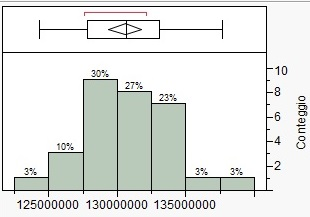
\includegraphics[]{./immagine/W100MBx100KB.jpg}
			\caption{Scrittura di un file di $100MB$ con blocchi di $100KB$}
			\label{fig:b-w100}
		\end{figure}
		In caso di distribuzioni skewed ed eventuali \emph{outlier}, si è optato per la mediana ed il SIQR.
				\begin{figure}[H]
			\centering
			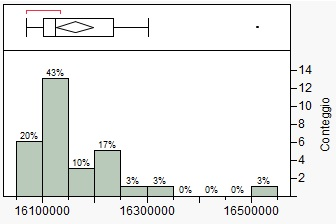
\includegraphics[]{./immagine/R1GBx1MB.jpg}
			\caption{Lettura di un file di $1GB$ con blocchi di $1MB$}
			\label{fig:b-r1}
		\end{figure}
		Sono stati quindi prodotti due data set, contenenti i dati delle operazioni di lettura e scrittura.
		\begin{figure}[H]
			\centering
			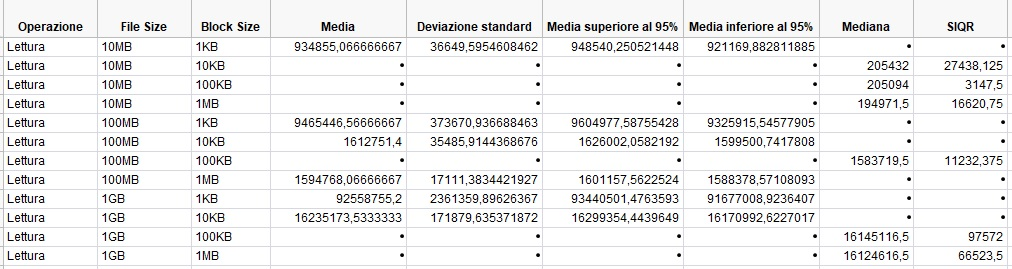
\includegraphics[width=17cm, height= 7cm]{./immagine/letture.jpg}
			\caption{Dati delle letture}
			\label{fig:b-r}
		\end{figure}
		\begin{figure}[H]
			\centering
			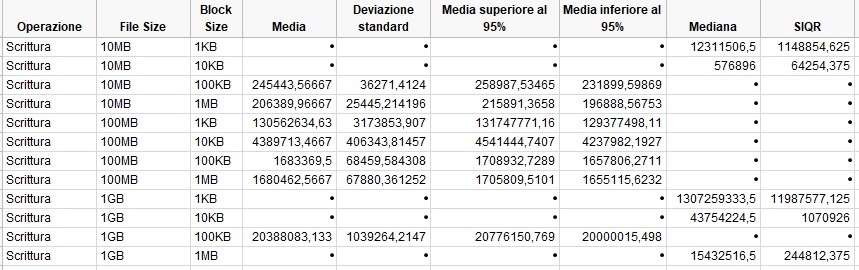
\includegraphics[width=17cm, height=7cm]{./immagine/scritture.jpg}
			\caption{Dati delle scritture}
			\label{fig:b-w}
		\end{figure}
		Si possono, inoltre, sfruttare i risultati ricavati per determinare la dimensione del campione necessaria per ottenere con accuratezza desiderata la media delle osservazioni con un certo livello di confidenza. Prendiamo in considerazione la scrittura di un file di $100MB$. I tempi medi stimati per effettuare l'operazione sono circa: $2.10min$ per blocchi di $1KB$, $4.4s$ per blocchi di $10KB$, $1.7s$ per blocchi di $100KB$, $1.7s$ per blocchi di $1MB$. Si può voler calcolare in questi casi un tempo accurato di $r=0.5\%$ con livello di confidenza del $95\%$. In questi casi, si ricaverebbe una media dei tempi accurata rispettivamente per al più di $6.5ds$, $22ms$, $8.4ms$, $8.4ms$. Si applica dunque:
		\begin{equation}
			n=\left( \frac{100zs}{r\bar{x}}\right) ^{2}
		\end{equation}
		con $z=1.96$, $s$ deviazione standard, $\bar{x}$ media. Si ottiene, quindi, il numero di punti necessari: $n=90$, $n=1316$, $n=254$, $n=250$.

\chapter{Dataset Reduction}

\section{Descrizione del problema}
Lo scopo di questo elaborato è quello di analizzare un set di dati e ridurlo, in modo che sia comunque rappresentativo della popolazione da cui è stato estratto il campione.\\
Il dataset in questione contiene informazioni riguardanti parametri e valori di prestazioni di un file system di Unix, raccolte in 3000 istanze, descritte da 24 feature.\\\\
L'obiettivo, quindi, sarà quello di selezionare un numero esiguo di righe, pur mantenendo la maggior percentuale di varianza e quindi di informazione possibile.\\
Per fare questo, dopo aver manipolato preliminarmente i dati, si sono utilizzate due tecniche: la \textbf{PCA} e il \textbf{Clustering}. Come software invece sono stati utilizzati JMP e Matlab.\\\\

\section{Trattamento preliminare dei dati}
Prima di utilizzare le tecniche sopracitate, è stata calcolata la varianza di ogni colonna con JMP e il risultato è stato il seguente:\\\\\\\\\\

\begin{figure}[!h]
	\centering
	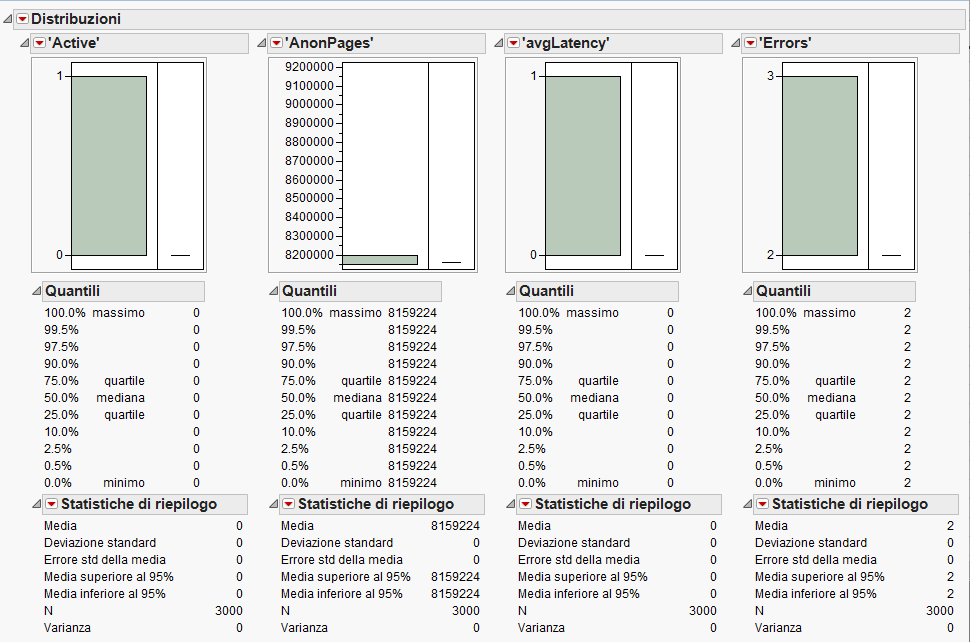
\includegraphics[width=15cm, height=10cm]{./immagine/colonne_costanti.png}
	\caption{Distribuzione colonne costanti}
	\label{fig:colonne_costanti}
\end{figure}

Come si nota sia dagli istogrammi e dal valore in basso, la varianza di queste colonne è nulla, quindi vengono eliminate in quanto non apportano contenuto informativo all'analisi dei dati.\\

\section{PCA}
Si è utilizzata la Principal Component Analysis per compiere una trasformazione lineare delle variabili originarie (gli attributi del dataset), proiettandole in un nuovo sistema cartesiano, in modo che le nuove variabili ottenute, dette \textbf{componenti principali} spieghino la maggior parte della varianza di quelle originarie.\\\\\\\\

\begin{figure}[!h]
	\centering
	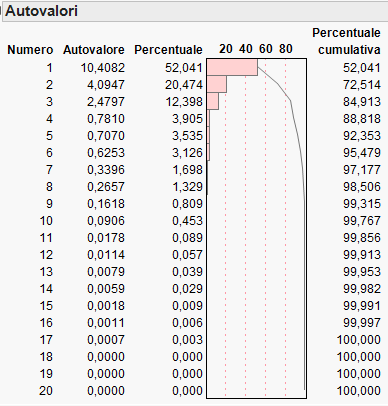
\includegraphics[width=12cm, height=10cm]{./immagine/autovalori.png}
	\caption{Componenti principali e varianza conservata}
	\label{fig:autovalori}
\end{figure}
Come si nota dalla figura esse sono ordinate in base a quanta varianza spiegano, quindi prendendo 6 componenti principali riesco a spiegare circa il 95\% della varianza.\\

\section{Clustering}
Una volta ridotto il numero di feature a 6 attraverso la PCA, si è ridotto il numero di istanze attraverso la tecnica del clustering. Quello che si fa è, una volta definita una metrica di distanza, di unire in gruppi i dati che hanno distanza minima, ovvero quelli che sono più simili.\\
Come metodo di clustering è stato scelto quello di \textbf{Ward}, che è una tecnica gerarchica agglomerativa che consiste nel formare cluster unendo ad ogni iterazione una coppia di cluster con l'obiettivo di minimizzare la varianza intra-cluster e massimizzare quella inter-cluster.\\
Il processo di clustering porta alla realizzazione della seguente struttura gerarchica detta \textbf{dendrogramma}:

\begin{figure}[!h]
	\centering
	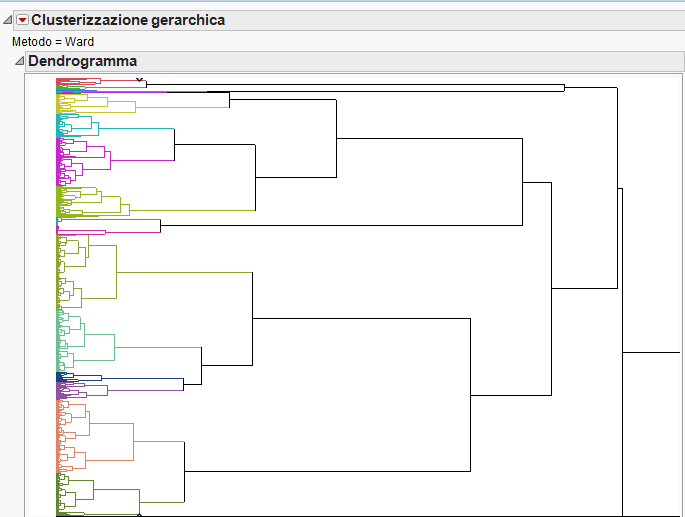
\includegraphics[width=15cm, height=12cm]{./immagine/dendrogramma.png}
	\caption{Dendrogramma}
	\label{fig:dendrogramma}
\end{figure}

Come si nota alla radice sono raggruppati tutti i dati in un unico cluster mentre, scendendo verso il basso i dati vengono divisi in più cluster fino a giungere alle foglie, che non sono altro che cluster formate da un solo elemento.\\ 
Più salgo verso la radice e più perdo varianza, più scendo verso le foglie e più la conservo, quindi bisogna trovare un trade-off tra la varianza persa e la riduzione del dataset.\\
La seguente immagine mostra la varianza persa a seconda del numero di cluster considerati:\\\\\\\\\\\\

\begin{figure}[!h]
	\centering
	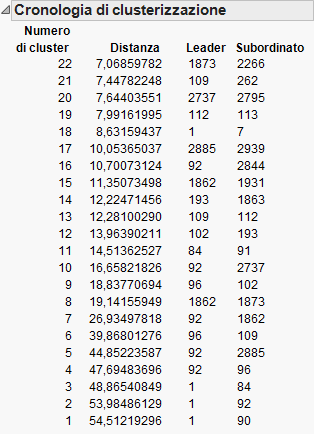
\includegraphics[width=8cm, height=10cm]{./immagine/cluster.png}
	\caption{Cluster con relativa varianza persa}
	\label{fig:cluster}
\end{figure}

In realtà si usa la devianza come metrica di distanza anzichè la varianza, in quanto vale la seguente relazione:
\begin{center}
	$devianza_{totale}=devianza_{intracluster}+devianza_{intercluster}$
\end{center} 
Quindi nella tabella precedente, ogni distanza indica la devianza persa considerando quel dato numero di cluster e calcolando il rapporto $\frac{devianza_{intracluster}}{devianza_{totale}}$, sono in grado di conoscere la percentuale di devianza e quindi di varianza (a meno di una costante) persa a seguito dell'operazione di clustering.\\\\
Si è scelto 19 come numero di cluster, poiché, superata tale soglia, si va a perdere troppa devianza cosi come si nota dal seguente grafico, dove sull'asse delle ascisse è stato messo il numero di cluster e sull'asse delle ordinate la distanza.\\\\\\\\

\begin{figure}[!h]
	\centering
	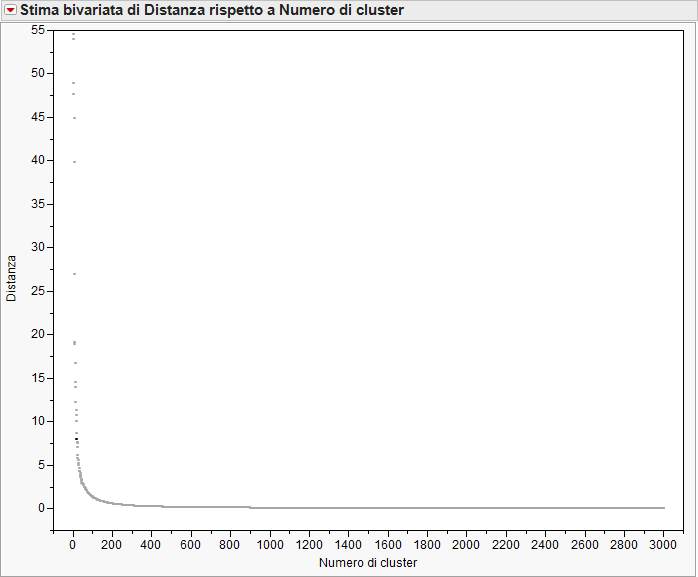
\includegraphics[width=10cm, height=10cm]{./immagine/grafico.png}
	\caption{Grafico devianza persa al variare del numero di cluster}
	\label{fig:grafico}
\end{figure} 

Scegliendo 19 cluster, quindi, perdiamo circa il 18,5\% della varianza del dataset originale e ne conservo l'81,5\%.\\\\\\\\\\\\\\\\\\\\\\

\section{Conclusioni}
In conclusione riportiamo il numero di dati che ogni cluster contiene con la relativa percentuale di copertura del dataset originario:\\

\begin{figure}[!h]
	\centering
	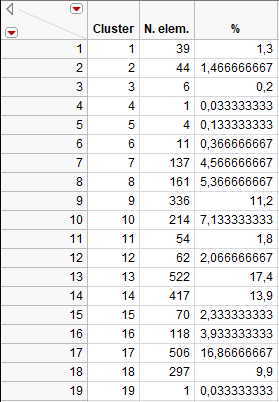
\includegraphics[width=8cm, height=10cm]{./immagine/cluster_size.png}
	\caption{Numero di elementi per ogni cluster}
	\label{fig:cluster_size}
\end{figure}

Come si nota dalla tabella ci sono alcuni cluster che contengono pochi elementi, ad esempio il cluster 19 ne contiene solo 1 e questo corrisponde all'istanza che presenta l'unico valore diverso da zero dell'attributo \textit{Slab}. Probabilmente in questi casi si tratta di \textbf{outlier}, cioè valori anomali, ma nonostante questo non sono stati eliminati in quanto potrebbero rappresentare un comportamento specifico del sistema preso in esame e quindi non avendo informazioni sulla loro significatività si è ritenuto opportuno mantenerli nel dataset.\\\\\\\\\\\\
Infine riportiamo i dati scelti in maniera casuale da ogni cluster (un elemento per ognuno), che sono rappresentativi del dataset originario.\\\\

\begin{figure}[!h]
	\centering
	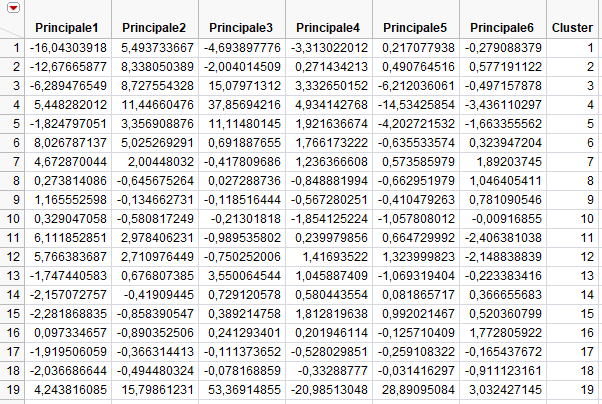
\includegraphics[width=15cm, height=13cm]{./immagine/final_data.png}
	\caption{Dati finali}
	\label{fig:final_data}
\end{figure}



\backmatter
% bibliography, glossary and index would go here.

\end{document}